\begin{figure}[htbp]
\centering

\includegraphics[width=0.95\linewidth]{manifold_geometry_plots.pdf}
\caption{(a) Hyperbolic grid mapping showing node density concentration at the surface ($z = 1.5$ m) with compactification parameter $\alpha_s = 0.05$. (b) Derivatives of Chebyshev basis polynomials $dT_n/dz$ showing spectral sensitivity at multiple scales.}
\label{fig:grid}
\end{figure}

\begin{figure}[htbp]
    \centering
    
\includegraphics[width=0.78\linewidth]{tier1_plane1.pdf}
    \caption{Diagnostic phase-space plot mapping Effective Modal Dimension ($D_{\mathrm{eff}}$) versus Wave Energy Fraction ($F_W$). Points represent individual 10-minute profiles and show the three-regime separation between continuous turbulence, wave-dominated states, and intermittent shear transitions.}
    \label{fig:phase_space}
\end{figure}

\begin{figure}[htbp]
    \centering
    
\includegraphics[width=0.78\linewidth]{tier1_plane2.pdf}
    \caption{Gradient stability versus structural profile geometry in the $(\mathrm{Ri}_g, \chi_N)$ plane. The distribution highlights how intermittent shear events occupy a high-curvature transition zone that is not cleanly captured by classical Richardson-number thresholds alone.}
    \label{fig:tier1_plane2}
\end{figure}

\begin{figure}[htbp]
\centering

\includegraphics[width=0.95\linewidth]{campaign_synoptic_evolution.pdf}
\caption{Continuous 240-hour timeline tracking 10-minute-averaged spectral features across the CASES-99 intensive observation window (22--31 October 1999). Top panel: Effective modal dimension $D_{\mathrm{eff}}$ trajectory. Bottom panel: Wave energy fraction $F_W$ tracking curve. Color-coded regions indicate GMM cluster membership by regime.}
\label{fig:synoptic_timeline}
\end{figure}

\begin{figure}[htbp]
\centering
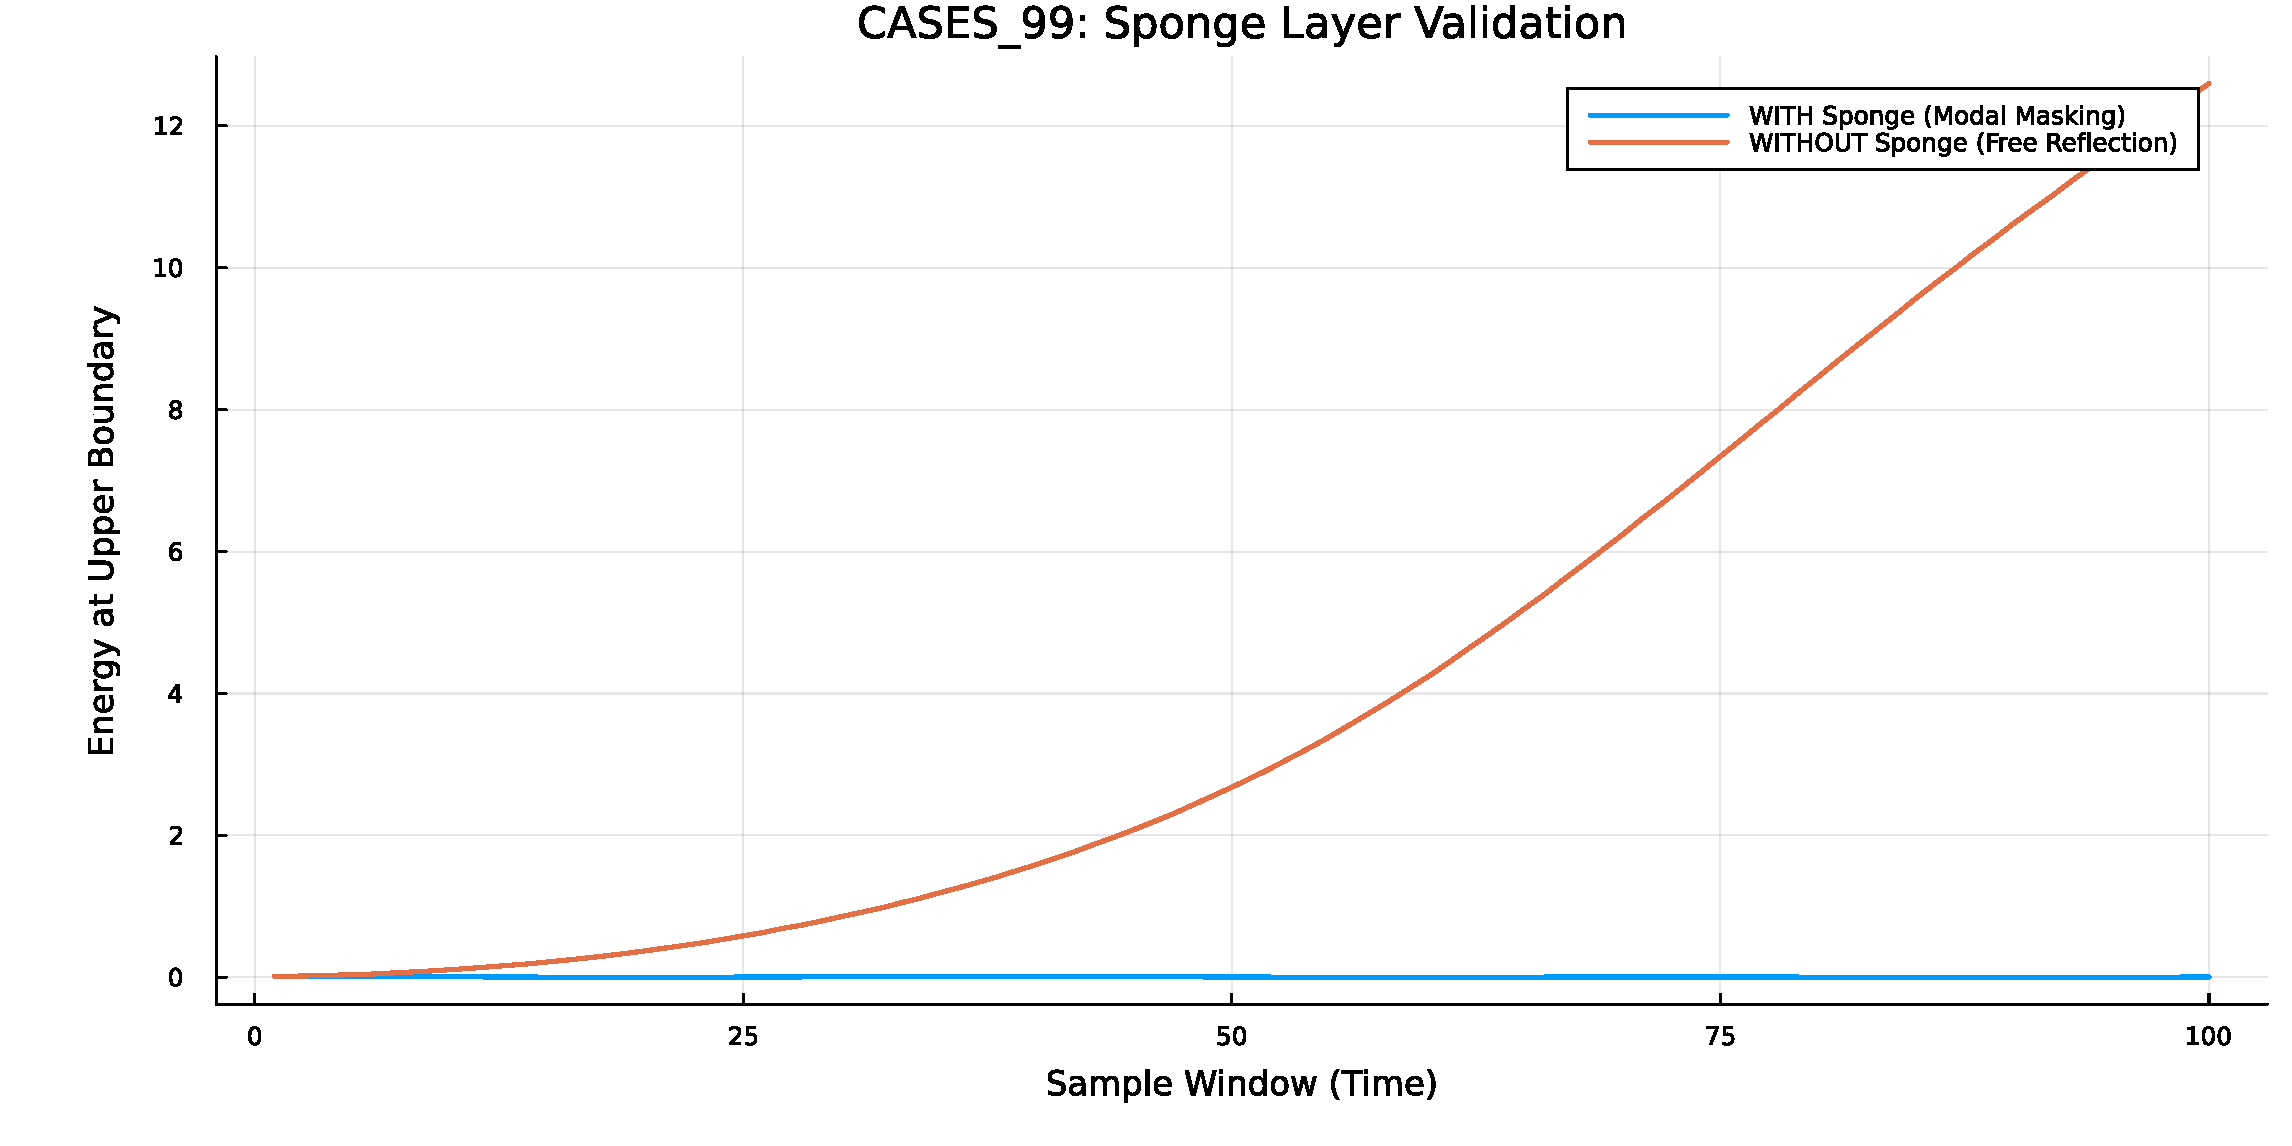
\includegraphics[width=0.85\linewidth]{../data/universal_sponge/cases_99/wave_reflection_test.pdf}
\caption{Sponge-layer wave reflection verification test tracking spatial decay of the normalized upward-propagating synthetic gravity wave amplitude as it approaches the upper boundary of the computational workspace ($z \to 55$ m). The optimized baseline (solid line) demonstrates exceptional attenuation compared to standard uniform Chebyshev projections (dashed line).}
\label{fig:sponge_test}
\end{figure}
